\documentclass{article}
\usepackage{amsmath}
\usepackage{amsfonts}
\usepackage{amssymb}
\usepackage{parskip}
\usepackage{multicol}
\usepackage{xcolor}
\usepackage{fancyhdr}
\usepackage{physics}
\usepackage{graphicx} % Required for inserting images
\newcommand{\matr}[1]{\mathbf{#1}}

\title{Honours Differential Equations}
\author{Notes by Christopher Shen}
\date{Winter 2023}

\begin{document}

\maketitle
\newpage

\tableofcontents
\newpage

\pagestyle{fancy}
\fancyhead{}
\fancyhead[L]{Honours Differential Equations}
\fancyhead[R]{Winter 2023}

\section{ODE systems}

\subsection{Integrating factors}
Consider linear DE of form
$$y'+P(x)y=Q(x)$$
Our integrating factor for this DE is:
$$I(x)=\exp\left(\int P(x)dx\right)$$
Then our solution is
$$y(x)=\frac{1}{I(x)} \int Q(x)I(x)dx + \frac{\alpha}{I(x)}$$
where here $\alpha$ is a constant.

\subsection{Change of variables}
For higher order differential equations of form $$y^{(n)} = F(y, y', \dots, y^{(n-1)}, t),$$
consider \textbf{change of variables} $x_{i+1} = y^{(i)}$ for $i \in \{0, 1, \dots, n-1\}$.
Then take derivative with respect to time to obtain a first order ODE system, which takes the form:
$$x_{j}'=F_j(t, x_1, \dots, x_n)$$ for $j=1, \dots, n$.
We either immediately write this as a matrix system or linearise near a critical point.

\subsection{Existence and uniqueness for IVPs}
An initial value problem ($\textbf{IVP}$) is defined as
$$\frac{dx}{dt} = f(x, t)$$ for $\textbf{initial}$ condition $x(t_0)=x_0$.
A solution $x:I \rightarrow$ $\mathbb{R}$ is a differentiable function that satisfies the IVP.
Similarly for a first order system $$x_{i}'=F_i(t, x_1, \dots, x_n)$$ to have a $\textbf{unique}$ solution,
$F_i$ and $\frac{\partial F_i}{\partial x_j}$
must be continuous in a region. Here $i, j \in \{1, \dots, n\}$.

\newpage

\subsection{Homogeneous systems}
Now consider $\boldsymbol{x}'=\matr{A}\boldsymbol{x}$, where $\matr{A}$ is a $n \times n$ matrix. \\
Substituting $\boldsymbol{x}=e^{rt} \boldsymbol{\xi}$ results in an eigenvector problem:
$$(\matr{A}-r_i \matr{I_n})\boldsymbol{\xi^{(i)}}=\boldsymbol{0}.$$
If eigenvalues repeat we try $\boldsymbol{x}=te^{rt} \boldsymbol{\xi}+e^{rt} \boldsymbol{\eta}$ which gives
$$(\matr{A}-r_i \matr{I_n})\boldsymbol{\eta^{(i)}}=\boldsymbol{\xi^{(i)}}.$$
The $\textbf{fundamental matrix}$ satisfies $\boldsymbol{\Psi}'=\matr{A}\boldsymbol{\Psi}$ and contains the basis of solutions. \\
$$\boldsymbol{\Psi}(t)=[\boldsymbol{x^{(1)}}, \dots, \boldsymbol{x^{(n)}}]$$
for $\boldsymbol{x^{(i)}} = \exp{(r_{\boldsymbol{i}} t)} \boldsymbol{\xi^{(i)}}$
and hence our general solution is $\boldsymbol{x}=\boldsymbol{\Psi} \boldsymbol{c}$. \\

\newpage
    
\subsection{Non-homogeneous systems}
Consider non-homogeneous ODE system:
$$\boldsymbol{x}'=\boldsymbol{A}\boldsymbol{x}+\boldsymbol{g}.$$
There a couple of different approaches we can take to solve such a system.
\begin{itemize}
    \item \textbf{Change of basis}
        
    Let $\boldsymbol{x}=\boldsymbol{T}\boldsymbol{y}$,
    where $\boldsymbol{T}$ is our eigenvector matrix from diagonalisation. \\
    So $\boldsymbol{A}=\boldsymbol{T}\boldsymbol{D}\boldsymbol{T}^{-1}$,
    and after some algebra we obtain:
    $$\boldsymbol{y}'=\boldsymbol{D}\boldsymbol{y}+\boldsymbol{T}^{-1}\boldsymbol{g}$$
    which can be solved by integrating factors. Finally revert back to $\boldsymbol{x}$.

    \item \textbf{Variation of parameters}

    So $\boldsymbol{x}_H=\boldsymbol{\Psi}\boldsymbol{c}$ solves the $\boldsymbol{x}'=\boldsymbol{A}\boldsymbol{x}$,
    where $\boldsymbol{c}$ is a constant vector.
        
    We then assume that the solution to our non-homogeneous system takes the form:
    $$\boldsymbol{x}=\boldsymbol{\Psi}\boldsymbol{u}$$
    for here $\boldsymbol{u} = \boldsymbol{u}(t)$. We then get $\boldsymbol{\Psi}\boldsymbol{u}'=\boldsymbol{g}$,
    which can be solved by eliminating variables and integrating.

    \item \textbf{Method of undetermined coefficients}

    Our non-homogeneous ODE system has solutions of form:
    $$\boldsymbol{x}=\boldsymbol{x}_H + \boldsymbol{x}_p$$

    Solving the homogeneous ODE gives us $\boldsymbol{x}_H$.
        
    On the other hand we just need to find a \textbf{particular solution}
    $\boldsymbol{x}_p$ that satisfies our non-homogeneous ODE. Then our solution is complete.

    Whilst the fastest, this method is not guaranteed to work.        
    \end{itemize}
    
\newpage

\subsection{Critical points \& linearisation}
Consider non-linear ODE system
$$x'=F(x, y),$$
$$y'=G(x, y).$$
We define $\boldsymbol{x^0}=\begin{bmatrix} x^0 \\ y^0 \end{bmatrix}$
as a \textbf{critical point} when $F(\boldsymbol{x^0})=G(\boldsymbol{x^0})=0$.

Non-linear systems may then be linearised by Taylor expanding them around a critical point $\boldsymbol{x^0}$,
and discarding higher order terms. \\
i.e. let $\boldsymbol{u}=\begin{bmatrix} u_1 \\ u_2 \end{bmatrix}$ where $u_1=x-x^0$ and $u_2=y-y^0$.
\begin{align*}
    \therefore u_1 '&= x' \\ &\approx F(x^0, y^0)+\left(\frac{\partial F}{\partial x}\right)_{x^0}(x-x^0)
    +\left(\frac{\partial F}{\partial y}\right)_{y^0}(y-y^0)
\end{align*}
\begin{align*}
    \therefore u_2 '&= y' \\ &\approx G(x^0, y^0)+\left(\frac{\partial G}{\partial x}\right)_{x^0}(x-x^0)
    +\left(\frac{\partial G}{\partial y}\right)_{y^0}(y-y^0)
\end{align*}
Then we end up with the following linear system:
$$\boldsymbol{u}' = \boldsymbol{A}\boldsymbol{u}$$
where $\boldsymbol{A}=\begin{bmatrix}
    \partial F/\partial x & \partial F/\partial y \\
    \partial G/\partial x & \partial G/\partial y
\end{bmatrix}_{\boldsymbol{x} = \boldsymbol{x^0}}$ and is a $2\times2$ Jacobian matrix. \\
    
Our critical points $\boldsymbol{x^0}$ may also be classified: \\
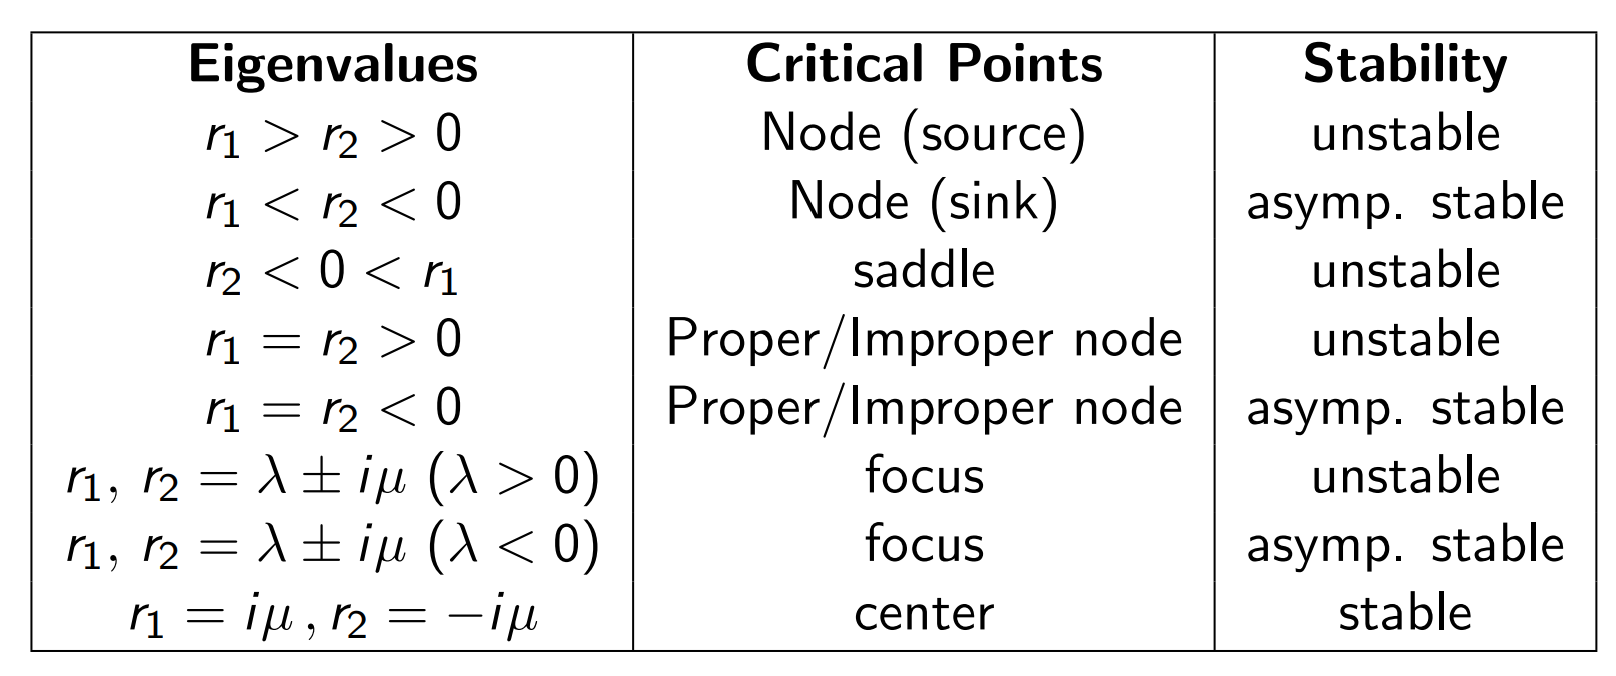
\includegraphics[scale=0.5]{f1.png}

Linearisation preserves critical point behaviour \textbf{except} when eigenvalues are of $r=\pm i\mu$ form,
for which then classification is unknown.

\newpage

\subsection{Stability of critical points}
\textbf{Stable} critical points $\boldsymbol{x^0}$: All solutions \underline{start} and \underline{stay near} $\boldsymbol{x^0}$.
    
$\forall \epsilon > 0; \exists \delta > 0; \forall \boldsymbol{x}_{solution}$ to $\boldsymbol{x}'=\boldsymbol{F}(\boldsymbol{x}, t)$: \\
$|\boldsymbol{x}(0)-\boldsymbol{x^0}|<\delta$ $\implies$ $|\boldsymbol{x}(t)-\boldsymbol{x^0}|<\epsilon$ for $\forall t \geq 0$ \\

\textbf{Attracting} critical points $\boldsymbol{x^0}$: All solutions \underline{tends} to $\boldsymbol{x^0}$.

$\forall \delta > 0:$ $|\boldsymbol{x}(0)-\boldsymbol{x^0}|<\delta$ $\implies$
$\displaystyle\lim_{t\rightarrow\infty} \boldsymbol{x}(t)=\boldsymbol{x^0}$ \\

\textbf{Asymptotically stable} critical points $\boldsymbol{x^0}$: Attracting \textbf{and} stable \\

\subsection{Lyapunov's theory and limit cycles}
In this section $\dot{\boldsymbol{x}}$ means its first time derivative. So consider:
$$\dot{x}=F(x, y),$$
$$\dot{y}=G(x, y)$$
defined in $\mathbb{R}^2$. Let $\boldsymbol{x^0} \in D$ be a critical point.
    
The function $E:D\subset\mathbb{R}^2\rightarrow\mathbb{R}$ is a Lyapunov function where 
$E(x^0, y^0)=0$, whenever it exists. Note that the time derivative of E is:
$$\frac{dE}{dt}=\frac{\partial E}{\partial x} F + \frac{\partial E}{\partial y} G$$
\begin{itemize}
    \item Let $E>0$ for $\forall \boldsymbol{x} \neq \boldsymbol{x^0}$.
        
    If $\frac{dE}{dt} \leq 0$ then $\boldsymbol{x^0}$ is stable.

    If $\frac{dE}{dt} < 0$ then $\boldsymbol{x^0}$ is asymptotically stable.

    \item If every neighbourhood of $\boldsymbol{x^0}$ contains $\boldsymbol{x^*}$ such that $E(\boldsymbol{x^*})>0$ \\
    \textbf{and} if $\frac{dE}{dt}>0$ then $\boldsymbol{x^0}$ is unstable.
    \end{itemize}
Now \textbf{limit cycles} are defined as periodic solutions such that at least one other \textcolor{red}{non-closed trajectory}
approaches the limit cycle as $t\rightarrow\infty$.

\newpage

\section{Fourier series}

\subsection{Real Fourier series}
Let $f(x)$ and $f'(x)$ be \textbf{piecewise continuous} in $[-L, L]$ with \textbf{period} $2L$. \\
i.e. $f(x)=f(x+\boldsymbol{2L})$ for $\forall x$. Then the Fourier series for $f(x)$ is
$$f_{FS}(x)=\frac{a_0}{2}+\sum_{n=1}^{\infty}(a_n \cos\frac{n\pi x}{L}+b_n \sin\frac{n\pi x}{L}).$$
The \textbf{convergence} of our Fourier series depends on the continuity of $f(x)$:
\begin{itemize}
    \item If $f(x)$ is \underline{continuous} then $f_{FS}(x)=f(x)$.
    \item If $f(\alpha)$ is \underline{discontinuous} then at point $\alpha$ we have
    $$f_{FS}(\alpha)=\frac{f(\alpha^{+})+f(\alpha^{-})}{2}.$$
\end{itemize} 
Note that $f(x)$ is continuous at $\alpha$ if $f(\alpha)=\displaystyle\lim_{x\rightarrow\alpha}f(x)$ and we define:
$$f(\alpha^-)=\displaystyle\lim_{x\rightarrow\alpha^-}f(x)$$ and
$$f(\alpha^+)=\displaystyle\lim_{x\rightarrow\alpha^+}f(x),$$
i.e. limits from left and right respectively. It is important to also note that the \underline{derivative} of a Fourier series is \textbf{not necessarily convergent}.
    
Now consider $S_n = \sin\frac{n\pi x}{L}$ and $C_n = \cos\frac{n\pi x}{L}$. We then have the following \textbf{orthogonality relations}:
$$\langle S_n, S_m \rangle=\langle C_n, C_m \rangle=L\delta_{mn}$$ and
$$\langle S_n, C_m \rangle=0$$
which are used to find $a_n$ and $b_n$ in $f_{FS}(x)$. So:
$$a_0=\frac{1}{L}\int_{-L}^{L}f(x)dx,$$
$$a_n=\frac{1}{L}\int_{-L}^{L}\cos\frac{n\pi x}{L}f(x)dx$$
and
$$b_n=\frac{1}{L}\int_{-L}^{L}\sin\frac{n\pi x}{L}f(x)dx.$$
    
Note that $\delta_{mn}$ is the \textbf{Kronecker delta} and is defined as:
$$\delta_{mn} =
\left\{
\begin{array}{ll}
	1  & \mbox{} m=n \\
	0 & \mbox{} m\neq n
\end{array}
\right.$$
These trigonometric identities are useful for finding Fourier coefficients:
$$\cos A\cos B = \frac{1}{2}[\cos(A-B)+\cos(A+B)],$$
$$\sin A\sin B = \frac{1}{2}[\cos(A-B)-\cos(A+B)],$$
$$\sin A\cos B = \frac{1}{2}[\sin(A+B)+\sin(A-B)].$$
The \textbf{inner product} of two functions is also defined as:
$$\langle u(x), v(x) \rangle=\int_{-L}^{L} u(x)v(x)dx.$$
A shortcut is to note that:
\begin{itemize}
    \item The Fourier series of \textbf{even} functions contains \underline{only} \textbf{cosines}.

    \item The Fourier series of \textbf{odd} functions contains \underline{only} \textbf{sines}.
\end{itemize}
\textbf{Even} functions are defined $f(-x)=f(x)$, and:
$$\int_{-L}^{L}f_{even}dx=2\int_{0}^{L}f_{even}dx.$$
Similarly \textbf{odd} functions are defined $f(-x)=-f(x)$, and:
$$\int_{-L}^{L}f_{odd}dx=0.$$

\newpage

\subsection{Complex Fourier series}
Our Fourier series may be rewritten as a $\textbf{complex Fourier series}$
$$f_{FS}(x)=\sum_{n=-\infty}^{\infty} c_n \exp\left(\frac{in\pi}{L} x\right)$$
using Euler's formula $e^{i\theta}=\sin{\theta}+i\cos{\theta}$. Then:
\[ c_n = \begin{cases} 
    (a_n - ib_n)/2 & n > 0 \\
    (a_0)/2 & n = 0 \\
    (a_n + ib_n)/2 & n < 0
\end{cases}\]
and therefore negative $n$ values are included. By orthogonality:
$$c_n=\frac{1}{2L}\int_{-L}^{L} \exp\left(-\frac{in\pi}{L} x\right) f(x)dx$$
for $\forall n \in \mathbb{Z}$. Here we define the \textbf{inner product} for complex functions as
$$\langle f, g\rangle=\int_{\alpha}^{\beta} f^*(x)g(x) dx$$
where $f^*(x)$ is the complex conjugate of $f(x)$. Then:
\begin{align*}
    \langle \exp\left(\frac{i\boldsymbol{m}\pi}{L} x\right), \exp\left(\frac{i\boldsymbol{n}\pi}{L} x\right)\rangle
    &=\int_{-L}^{L} \exp\left(-\frac{i\boldsymbol{m}\pi}{L} x\right) \exp\left(\frac{i\boldsymbol{n}\pi}{L} x\right)dx \\
    &= 2L\delta_{mn}
\end{align*}
and since $f(x)=f_{FS}(x)$ we obtain our formula.

\subsection{Parseval's theorem}
Parseval's theorem states that given a periodic $f(x)$ with convergent Fourier series
we have that
\begin{align*}
    \langle f, f\rangle
    &=\int_{-L}^{L} |f(x)|^2 dx \\
    &=2L\sum_{n=-\infty}^{\infty} |c_n|^2 \\
    &=L\left[ \frac{|a_0|^2}{2} + \sum_{n=1}^{\infty} (|a_n|^2 + |b_n|^2)\right]
\end{align*}
and is derived by orthogonality and direct calculation.

\newpage

\section{PDEs}

\subsection{Separation of variables}
The only methodology considered is separation of variables. So for PDE:
$$\hat{D}[u(x_1,\dots,x_n)]=0$$
where $\hat{D}$ is our differential operator, we look for solutions of form:
$$u(x_1,\dots,x_n)=X_1(x_1)\cdots X_n(x_n)$$
subject to \textbf{initial} and \textbf{boundary} conditions.

\subsection{Heat equation}
The heat equation is an equation of the following form:
$$\frac{\partial u}{\partial t}=\alpha^2\frac{\partial^2 u}{\partial x^2}.$$
where $\alpha^2$ is the thermal diffusivity constant. 

\subsubsection{Standard boundary conditions}
We firstly define:
\begin{itemize}
    \item \textbf{Initial condition}: $u(x,0)=f(x)$ for $0\leq x\leq L$

    \item \textbf{Boundary condition}: $u(0,t)=u(L,t)=0$ for $\forall t>0$
\end{itemize}
Let solutions be of form:
$$u(x,t)=X(x)\cdot T(t)$$
$$\therefore X(x)\cdot \dot{T}(t)=\alpha^2 X''(x)\cdot T(t)$$
Only a constant function may satisfy the first equality:
$$\frac{1}{\alpha^2}\frac{\dot{T}}{T}=\frac{X''}{X}=-\lambda.$$
Writing this as two ODEs:
$$\dot{T}+\alpha^2\lambda T=0$$
$$X''+\lambda X=0.$$
The first one we can directly integrate, yielding:
$$T(t)=a_1\exp\left(-\alpha^2\lambda t\right).$$
The second ODE is a spring system, hence it has solution of form:
$$X(x)=b_1\cos\lambda^{1/2} x+b_2\sin\lambda^{1/2} x.$$

\newpage

However this time before proceeding we need to \underline{consider}
\underline{boundary conditions}:
$$X(0)=X(L)=0.$$
We find $X(0)=b_1=0$ and $X(L)=b_2\sin\lambda^{1/2} L=0$.

The second equation implies that $\lambda$ must of the following form:
$$\lambda_n=\left(\frac{n\pi}{L}\right)^2
\hspace{0.1in}\text{for}\hspace{0.1in}\forall n\in\mathbb{N}$$
and so
$$X''+\lambda X=0\implies X_n=b_2\sin\lambda_n^{1/2} x.$$
Since $\lambda$ is discretised:
$$\therefore T_n=a_1\exp\left(-\alpha^2\lambda_n t\right).$$
Our general solution must then be:
$$u(x,t)=\sum_{n=1}^{\infty}c_n\exp\left(-\alpha^2\lambda_n t\right)
\sin\lambda_n^{1/2} x$$
where $\lambda_n=\left(\frac{n\pi}{L}\right)^2$. Using initial condition $u(x,0)=f(x)$:
$$f(x)=\sum_{n=1}^{\infty}c_n\sin\lambda_n^{1/2} x$$
and we recognise this as an \underline{odd} Fourier series with period $2L$.
$$\therefore\int_{-L}^{L}\sin(\lambda_n^{1/2} x) f(x)dx=\sum_{n=1}^{\infty}c_n\int_{-L}^{L}\left(
\sin(\lambda_n^{1/2} x)\right)^2dx$$
$$\therefore2\int_{0}^{L}\sin(\lambda_n^{1/2} x) f(x)dx
=c_n L$$
The final step we split the integration range and use $x=-x^*$.
$$\therefore c_n=\frac{2}{L}\int_{0}^{L}\sin(\lambda_n^{1/2} x) f(x)dx$$
This is fine because we can extend $u(x,t)$ via \underline{reflection} for negative $x$.

\newpage

\subsubsection{Fixed boundary temperatures}
We reconsider the heat equation:
$$\frac{\partial u}{\partial t}=\alpha^2\frac{\partial^2 u}{\partial x^2}$$
but now with the following \textbf{non-homogeneous boundary conditions}:
\begin{itemize}
    \item $u(0,t)=T_1$
    \item $u(L,t)=T_2$
    \item $u(x,0)=f(x)$
\end{itemize}
Physically our rod has fixed boundary temperatures, namely $T_1$ and $T_2$.

We approach this problem with a change of variables:
$$v(x)=\lim_{t\rightarrow\infty}u(x,t).$$
Using our boundary conditions $v$ must be linear:
$$\therefore v(x)=\frac{T_2-T_1}{L}x+T_1$$
since $v''=0$, $v(0)=T_1$ and $v(L)=T_2$. We then deduce that:
$$u(x,t)=v(x)+\omega(x,t)$$
for $\omega(x,t)$ satisfies the same heat equation with initial conditions:
\begin{itemize}
    \item $\omega(0,t)=\omega(L,t)=0$
    \item $\omega(x,0)=f(x)-v(x)$
\end{itemize}
Recognising this as our initial example:
$$\omega(x,t)
=\sum_{n=1}^{\infty}c_n\exp\left(-\alpha^2\lambda_n t\right)
\sin\lambda_n^{1/2} x$$
where again $\lambda_n=\left(\frac{n\pi}{L}\right)^2$ and because $\omega(x,t)$ is a Fourier series with period $2L$:
$$c_n=\frac{2}{L}\int_{0}^{L}\sin(\lambda_n^{1/2} x)\{f(x)-v(x)\} dx.$$

\newpage

\subsubsection{Insulated rod ends}
For the final example we consider:
$$\frac{\partial u}{\partial t}=\alpha^2\frac{\partial^2 u}{\partial x^2}$$
and define the following conditions:
\begin{itemize}
    \item $\displaystyle\frac{\partial}{\partial x}u(0,t)
    =\displaystyle\frac{\partial}{\partial x}u(L,t)=0$
    \item $u(x,0)=f(x)$
\end{itemize}
We begin again with a separation of variables:

\newpage

\subsection{Wave equation}

\newpage

\subsection{Laplace's equation}
Laplace's equation takes the form $\boldsymbol{\nabla}^2 u=0$. In two dimensions:
$$\frac{\partial^2 u}{\partial x^2}+\frac{\partial^2 u}{\partial y^2}=0$$
and we only consider boundary conditions. (Dirichlet conditions)

\subsubsection{Rectangular boundary conditions}
We open with the following example:
\begin{itemize}
    \item \textbf{Boundary for y}: $u(x,0)=u(x,b)=0$

    \item \textbf{Boundary for x}: $u(0,y)=0$ and $u(a,y)=f(y)$
\end{itemize}
where $x\in[0,a]$ and $y\in[0,b]$.
Begin by separation of variables:
$$u(x,y)=X(x)\cdot Y(y)$$
$$\therefore\frac{X''}{X}=-\frac{Y''}{Y}=\lambda.$$
Recognising the previous statement as two ODEs:
$$X''-\lambda X=0\hspace{0.05in}
\text{for}\hspace{0.05in}X(0)=0$$
$$Y''+\lambda Y=0\hspace{0.05in}\text{for}
\hspace{0.05in}Y(0)=Y(b)=0$$
The second ODE we have already solved in the heat equation. It has solution:
$$Y_n=a_1\sin(\lambda_n^{1/2} y)\hspace{0.05in}
\text{for}\hspace{0.05in}\lambda_n=\frac{n^2\pi^2}{b^2}.$$
The first ODE has solutions of form:
$$X_n=a_2\cosh(\lambda_n^{1/2}x)
+a_3\sinh(\lambda_n^{1/2}x)$$
where these are the hyperbolic functions:
$$\sinh x=\frac{1}{2}(e^x-e^{-x})$$
$$\cosh x=\frac{1}{2}(e^x+e^{-x}).$$
Using our boundary condition $X(0)=0$ gives:
$$X_n=a_3\sinh(\lambda_n^{1/2} x).$$
Now putting all of this together we get:
$$u(x,y)=\sum_{n=1}^{\infty}c_n\sinh(\lambda_n^{1/2} x)
\sin(\lambda_n^{1/2} y)$$

\newpage

To find coefficients $c_n$ we use $u(a,y)=f(y)$.
$$\therefore f(y)=\sum_{n=1}^{\infty}c_n\sinh(\lambda_n^{1/2} a)
\sin(\lambda_n^{1/2} y)$$
Since we have a Fourier series with period $2b$:
\begin{align*}
    \int_{-b}^{b}\sin(\lambda_n^{1/2} y)f(y)dy
    &=\sum_{n=1}^{\infty}c_n\sinh(\lambda_n^{1/2} a)
    \int_{-b}^{b}\sin(\lambda_n^{1/2} y)dy \\
    &=c_n\sinh(\lambda_n^{1/2} a)\cdot b
\end{align*}
We can split the first integral to give us:
$$c_n=\frac{2}{b\sinh(\lambda_n^{1/2} a)}
\int_{0}^{b}\sin(\lambda_n^{1/2} y)f(y)dy$$
where $\lambda_n=\left(\frac{n\pi}{b}\right)^2$
and our solution is complete.

\subsubsection{Circular boundary conditions}
Now we solve Laplace's equation
$$\frac{\partial^2 u}{\partial x^2}+\frac{\partial^2 u}{\partial y^2}=0$$
but with a circular boundary. In polar coordinates $(r,\theta)$:
\begin{itemize}
    \item $u(a,\theta)=f(\theta)$
    \item $u(r,\theta)$ is bounded
\end{itemize}
where $a$ is the radius of our circle and $\theta\in[0,2\pi]$. Since $u=u(x,y)$:
$$u'_{\theta}=u'_x x'_{\theta}+u'_y y'_{\theta}$$
$$u''_{\theta\theta}=(u''_{xx}x'_{\theta}+u''_{xy}y'_{\theta})x'_{\theta}
+u'_x x''_{\theta\theta}+(u''_{yy}y'_{\theta}+u''_{xy}x'_{\theta})x'_{\theta}+u'_y y''_{\theta\theta}$$
$$u'_r=u'_x x'_r+u'_y y'_r$$
$$u''_{rr}=(u''_{xx}x'_r+u''_{xy}y'_r)x'_r
+u'_x x''_{rr}+(u''_{xy}x'_r+u''_{yy}y'_r)y'_r+u'_y y''_{rr}$$
and here we have used the chain rule.

\newpage

Applying these derivatives we obtain the following equation:
$$\frac{\partial^2 u}{\partial r^2}+\frac{1}{r^2}\frac{\partial^2 u}{\partial\theta^2}
+\frac{1}{r}\frac{\partial u}{\partial r}=0.$$
Using separation of variables:
$$u(r,\theta)=R(r)\Theta(\theta)$$
$$\therefore r^2\frac{R''}{R}+r\frac{R'}{R}=-\frac{\ddot{\Theta}}{\Theta}=\lambda$$
where $\lambda$ is our separation constant.
$$\therefore\ddot{\Theta}+\lambda\Theta=0$$
$$\therefore r^2 R''+rR'=\lambda R$$

\newpage

\section{Sturm-Liouville theory}

\subsection{Regular S-L problems}
Sturm-Liouville theory is a general theory for 2nd order ODEs.

Consider the following eigenvalue ODE:
$$-\dv{x}\left(p(x)\dv{y}{x}\right)+q(x)y=\lambda r(x)y$$
where $r(x)$ is our \underline{weight function}.
We define the following boundary conditions:
\begin{enumerate}
    \item $a_1 y(0)+a_2 y'(0)=0$

    \item $b_1 y(1)+b_2 y'(1)=0.$
\end{enumerate}
This is a \textbf{regular Sturm-Liouville} problem, where $p(x)$, $p'(x)$, $q(x)$, $r(x)$ are \underline{continuous} functions and $p(x)$, $r(x)$ are \underline{strictly positive} functions for $\forall x\in[0,1]$.

\textbf{Eigenvalues} $\lambda_n$ yield \textbf{eigenfunctions} $\phi_n(x)$
which are \underline{nontrivial solutions} to our S-L problem. Important consequences include:
\begin{itemize}
    \item Eigenvalues $\lambda_n$ of a S-L problem are \textbf{real}. 
    
    Furthermore each eigenvalue corresponds to one eigenfunction.

    \item Eigenfunctions $\phi_n(x)$ are \underline{orthogonal}:
    $$\langle \phi_m,\phi_n \rangle
    =\int_{0}^{1}r(x)\phi_m(x)\phi_n(x) \dd x=\delta_{mn}$$
    in Hilbert space $L^2([0,1],r(x)\dd x)$.
\end{itemize}

Note that our eigenfunctions are orthonormal and so we define:
$$\phi_n(x)=k_n y_n(x)$$
where $k_n$ is our scale factor.
Since $\langle \phi_n,\phi_n \rangle=1$:
$$\therefore\int_{0}^{1}r(x)k_n^2y_n^2(x)\dd x=1$$
and so we have that:
\begin{align*}
    k_n
    &=\frac{1}{\sqrt{\langle y_n,y_n \rangle}} \\
    &=\Bigl(\int_{0}^{1}r(x)y_n^2(x)\dd x\Bigl)^{-1/2}.
\end{align*}

\newpage

\subsubsection{General 2nd order ODEs}
Consider the following general 2nd order eigenvalue ODE:
$$-P(x)\dv[2]{y}{x}-\omega(x)\dv{y}{x}+q(x)y=\lambda r(x)y.$$
Multiply this by the following integrating factor:
$$F(x)=\exp\Bigl[\int_{0}^{x}
\frac{\omega(s)-p'(s)}{p(s)}\dd s\Bigl]$$
yields an ODE of S-L form:
$$-\dv{x}\Bigl[F(x)P(x)\dv{y}{x}\Bigl]
+F(x)q(x)y=\lambda F(x)r(x)y.$$

\subsubsection{Lagrange's identity}
Our previous definition is motivated by the \textbf{Lagrange's identity}:
\begin{align*}
    \langle \mathcal{L}[u], v \rangle - \langle u, \mathcal{L}[v] \rangle
    &=-\Bigl[p\Bigl(u'v^*-u(v^*)'\Bigl)\Bigl]_{0}^{1} \\
    &=-\Bigl[p(x)(\dv{u}{x}\cdot v^*-u\cdot\dv{v^*}{x})\Bigl]_{0}^{1}
\end{align*}
where $u=u(x)$, $v=v(x)$ are \underline{complex} functions and
$$\mathcal{L}[u]=-\dv{x}\Bigl[p(x)\dv{u}{x}\Bigl]+q(x)u.$$
Here the inner product is defined as
$$\langle u,v \rangle=\int_{0}^{1}uv^* \dd x$$
and we have integrated by parts using the following identities:
$$\bigl[pu'v^*\bigl]'=\bigl(pu'\bigl)'v^*+pu'(v^*)'$$
$$\bigl[pu(v^*)'\bigl]'=\Bigl(p(v^*)'\Bigl)'u+pu'(v^*)'.$$
For a S-L problem its properties follow from:
$$\langle \mathcal{L}[u], v \rangle=\langle u, \mathcal{L}[v] \rangle$$
where functions $u$ and $v$
satisfy its \underline{boundary conditions}.

\newpage

\subsubsection{Series expansion}
Now the set of orthonormal eigenfunctions $\{\phi_n(x)\}$
from a S-L problem with boundary conditions
may be used to expand function $f(x)$:
$$f_\phi(x)=\sum_{n=1}^{\infty} c_n\phi_n(x)$$
for $\forall x\in[0,1]$. Integrating this on both sides:
\begin{align*}
    \int_{0}^{1}r(x)\phi_m(x)f(x)\dd x
    &=\int_{0}^{1}r(x)\phi_m(x)
    \sum_{n=1}^{\infty} c_n\phi_n(x)\dd x \\
    &=\sum_{n=1}^{\infty} c_n
    \int_{0}^{1}r(x)\phi_m(x)\phi_n(x)\dd x \\
    &=\sum_{n=1}^{\infty} c_n\delta_{mn} \\
    &=c_m
\end{align*}
and so we get a general formula for our coefficients:
$$c_n=\int_{0}^{1}r(x)\phi_n(x)f(x)\dd x.$$
If $f(x)$ and $f'(x)$ are \underline{piecewise continuous}
on $x\in[0,1]$ then:
$$\forall x\in(0,1);\sum_{n=1}^{\infty} c_n\phi_n(x)
=\frac{f(x^-)+f(x^+)}{2}$$
where these are the left and right handed limits.

\newpage

\subsection{Non-homogeneous S-L problems}
Consider:
$$\mathcal{L}[y]=\mu r(x)y+f(x)$$
where $f(x)$ is our non-homogeneous term, and that we define
$$\mathcal{L}[y]=-\dv{x}\Bigl[P(x)\dv{y}{x}\Bigl]+q(x)y.$$
Given that this ODE satisfies the S-L boundary conditions:
$$\mathcal{L}[y]=\lambda r(x)y$$
is solved by a sum of eigenfunctions
$$y(x)=\sum_{n=1}^{\infty} b_n\phi_n(x).$$
Substituting this into our original ODE gives:
\begin{align*}
    \sum_{n=1}^{\infty}b_n\mathcal{L}[\phi_n(x)]
    &=r(x)\sum_{n=1}^{\infty}b_n\lambda_n\phi_n(x) \\
    &=\mu r(x)\sum_{n=1}^{\infty}b_n\phi_n(x)+f(x).
\end{align*}
Rearranging then gives:
$$\frac{f(x)}{r(x)}=\sum_{n=1}^{\infty}
b_n(\lambda_n-\mu)\phi_n(x).$$
Now we can also expand $\displaystyle\frac{f(x)}{r(x)}$
in terms of our eigenfunctions:
$$\frac{f(x)}{r(x)}=\sum_{n=1}^{\infty}c_n\phi_n(x)$$
with
\begin{align*}
    c_n
    &=\int_{0}^{1}r(x)\phi_n(x)
    \frac{f(x)}{r(x)} \dd x \\
    &=\int_{0}^{1}\phi_n(x)f(x)\dd x
\end{align*}
and so equating yields the following relation
$$b_n=\frac{c_n}{\lambda_n-\mu}.$$

\newpage

\subsection{Singular S-L problems}
quite alot of theory not covered in this course

general definition of singular s-l problems

bessel's equation (order 0 example)

conditions for singular problems

\newpage

\subsection{S-L Series solutions}

\newpage

\section{Laplace transforms}

\end{document}